\chapter{Elliptic Curve Cryptography}
Abbiamo visto come la sicurezza può essere affidata ad aspetti computazionali o logici (per teoremi matematici ecc). Per quanto riguarda la \textit{computational security} abbiamo osservato due principi fondamentali: \textbf{Discrete-Logarithm} (\cref{prop:disclog}) e \textbf{Prime-Factorization} (\cref{prop:prodfact}).\\
E' stato osservato che a seconda del gruppo usato nella crittografia, questi problemi possono essere più o meno complessi da risolvere. In particolare, alcuni dati sul tempo usato per risolvere il problema di \textbf{DLog} sono i seguenti:
\begin{itemize}
    \item \textbf{Dlog in $Z^*(p)$:} $\exp{O(n^{\frac{1}{3}})}$.
    \item \textbf{Dlog in EC:} $\exp{O(n^{\frac{1}{2}})}$.
    \item \textbf{Dlog in $(Z(p),+)$:} polinomial-time
\end{itemize}
\begin{note}
Il fattore di scala $n$ è la \textbf{dimensione} degli elementi nel campo. Le curve ellittiche sono quelle che scalano meglio, per questo vengono usate.
\end{note}
\section{EC Minor Details}
Le curve ellittiche non sono delle vere ellissi. Sono delle curve generate dalla \textbf{Espressione di Weierstrass}:
\begin{definition}[Weierstrass Equation for EC]\label{def:weiereq}
Una curva ellittica è descritta dal seguente sistema:
\begin{equation}\label{eq:weiereq}
    \begin{cases}
    y^2=x^3+ax+b\\
    4a^3+27b^2\ne0
    \end{cases}
\end{equation}
\end{definition}
\begin{figure}[h]
\vspace{-10pt}
     \centering
     \begin{subfigure}[b]{0.3\textwidth}
         \centering
         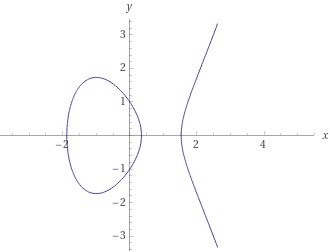
\includegraphics[width=\textwidth]{image/ecc/ec1.png}
         \caption{$y^2=x^3-3x+1$}
         \label{fig:ec1}
     \end{subfigure}
     \hfill
     \begin{subfigure}[b]{0.3\textwidth}
         \centering
         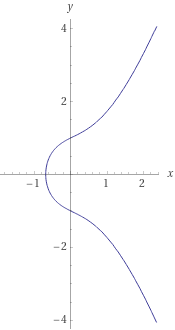
\includegraphics[width=0.4\textwidth]{image/ecc/ec2.png}
         \caption{$y^2=x^3+x+1$}
         \label{fig:ec2}
     \end{subfigure}
     \hfill
        \begin{subfigure}[b]{0.3\textwidth}
         \centering
         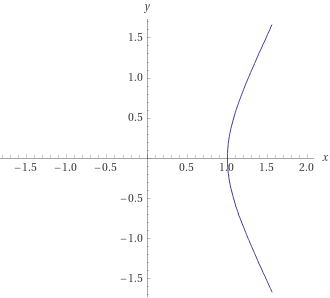
\includegraphics[width=0.9\textwidth]{image/ecc/ec3.png}
         \caption{$y^2=x^3-1$}
         \label{fig:ec3}
     \end{subfigure}
        \caption{ECC examples}
        \label{fig:ecc}
\end{figure}
Per trasformare le EC in un gruppo, definiamo un operatore che sia omomorfico, basandoci sul prossimo teorema:\pagebreak
\begin{theorem}[General Rule for EC]\label{thm:ecrule}
Se tre punti di una curva ellittica risiedono sulla stessa retta allora la loro somma è nulla.
\end{theorem}
\begin{figure}[h]
    \centering
    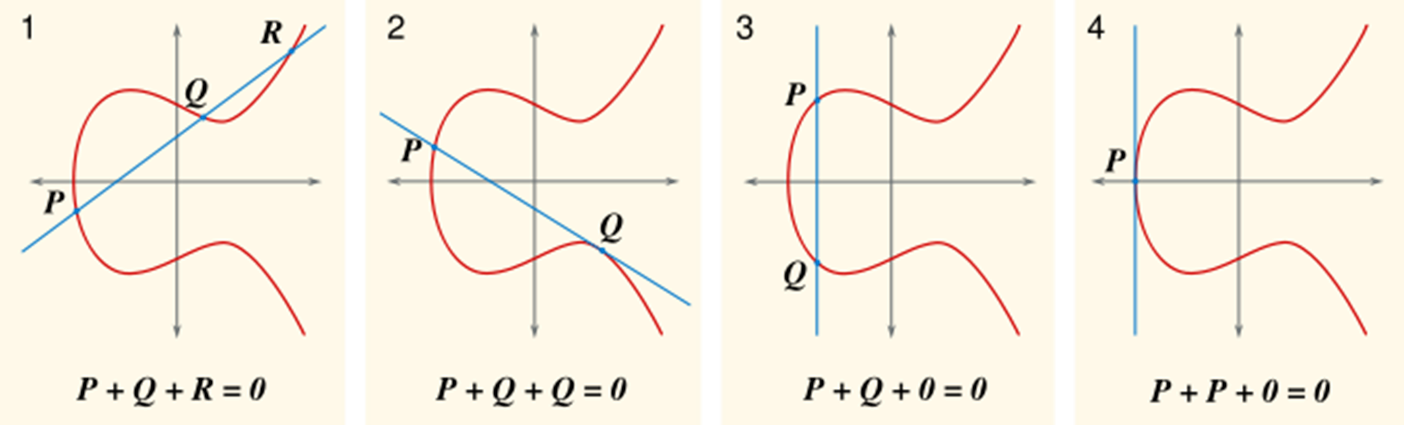
\includegraphics{image/ecc/ecrule.png}
    \caption{EC General Rule}
    \label{fig:ecrule}
\end{figure}
Allora, definiamo l'operatore:
\begin{definition}[EC "Sum" Operator]\label{def:ecsum}
Sia $+$ il nome dell'operatore e $P,Q,R$ dei punti sulla curva tali che $P+Q=R$. Allora:
\begin{itemize}
    \item $P\ne Q$: tracciare la retta passante per $P$ e $Q$. Il punto di intersezione con la curva è $-R$. Invertendo il segno otteniamo $R$.
    \item $P=Q$: tracciare la tangente alla curva in $P$. $-R$ è il punto di intersezione con la curva. Invertendo il segno otteniamo $R$.
    \item $-P=Q$: completiamo l'insieme dei punti della curva con una \textbf{"Chiusura all'Infinito"}, aggiungendo il punto $0$. Allora $P+0=P$
\end{itemize}
\end{definition}
Questa definizione ci permette di rispettare le richieste sulla chiusura dell'operatore.\\
Possiamo dedurre delle relazioni algebriche per definire in modo rigoroso l'operatore di somma.
\begin{theorem}[Algebric Relationships in EC]\label{thm:ecalg}
Siano $P=(x_1,y_1),Q=(x_2,y_2)$. Allora $R=P+Q=(x_3,y_3)$. Allora:
\begin{equation}\label{eq:ecalg}
    \begin{aligned}
    x_3&=\lambda^2-x_1-x_2\\
    y_3&=\lambda(x_1-x_3)+y_1\\
    \lambda&=\begin{cases}
    \frac{y_2-y_1}{x_2-x_1}&P\ne Q\\
    \frac{3x_1^2+a}{2y_1}&P=Q
    \end{cases}
    \end{aligned}
\end{equation}
\end{theorem}
\begin{proof}
Siano $P=(x_1,y_1),Q=(x_2,y_2)$. Allora $R=P+Q=(x_3,y_3)$.
\begin{itemize}
    \item $P\ne Q$: l'equazione della retta passante per due punti è:
    \begin{equation}\label{eq:rect}
    y=y_1+\frac{y_2-y_1}{x_2-x_1}(x-x_1)=\lambda(x-x_1)+y_1    
    \end{equation}
    Messa a sistema con la \cref{eq:weiereq} troviamo che: $(\lambda(x-x_1)+y_1)^2=x^3+ax+b$.\\
    Espandendo e portando tutto ad un membro troviamo un espressione del tipo: $x^3-\lambda^2x^2+\dots=0$.
    Poiché il termine di sinistra è un polinomio di terzo grado e \textbf{per costruzione del problema} conosciamo 2 soluzioni su 3, allora possiamo affermare che avrà una fattorizzazione del tipo: 
    \[(x-x_1)(x-x_2)(x-x_3)=x^3-(x_1+x_2+x_3)x^2+\dots
    \]
    Quindi: $\lambda^2=x_1+x_2+x_3\longrightarrow x_3=\lambda^2-x_1-x_2$. Trovare $y_3$ è adesso elementare, basta sostituire in \cref{eq:rect} e cambiare il segno.
    \item $P=Q$: L'equazione del fascio di rette per un punto è:
    \begin{equation}\label{eq:rectspan}
        y=y_1+k(x-x_1)=\lambda(x-x_1)+y_1
    \end{equation}
    Derivando l'equazione della curva troviamo:
    \[
    2y\frac{dy}{dx}=3x^2+a\longrightarrow\frac{dy}{dx}=\frac{3x^2+a}{2y}
    \]
    Allora: $\lambda=k=\frac{3x_1^2+a}{2y_1}$
\end{itemize}
\end{proof}
\section{EC over $\mathcal{Z}(p)$}
L'interpretazione geometrica usata fino ad ora è valida per i numeri reali. Consideriamo adesso però l'insieme costituiti dagli \textit{interi in modulo $p$}: le coordinate dei punti della curva saranno degli interi in $\mathcal{Z}(p)$ tali che:
\begin{equation}\label{eq:validecc}
    y^2\bmod{p}=x^3+ax+b\bmod{p}
\end{equation}
Questo significa che il numero di punti ammissibili è un insieme limitato, non più $p^2$ ma $p-1$ più lo zero, ovvero $p$ punti.
\begin{example} Consideriamo il gruppo descritto da $x^3+x+1\bmod5$. Prendiamo allora le coppie $(i,j),\,i,j\in[0,4]$ tali che $j^2=i^3+i+1\bmod5$ e il punto 0.\\
Per $x=1$ troviamo $y=3$. Se il punto $P=(1,3)$ è sulla curva, allora ne soddisfa l'equazione e ciò implicherebbe che esiste un numero \textbf{intero} il cui quadrato è 3: 
\[3^2\bmod5=1^3+1+1\bmod5\longrightarrow4=3\]
Poiché la relazione precedente è falsa deduciamo che il punto $(1,3)$ non appartiene al nostro gruppo.\\
Per $x=0$ invece troviamo $0^3+0+1=1$ e la relazione della curva è banalmente verificata perché $1^2=1$, quindi il punto $P=(0,1)$ appartiene al gruppo.\\
Ciclando su tutte le coppie possiamo vedere che dei 25 punti possibili soltanto 8+1 sono i punti effettivamente nel gruppo. In particolare:
\[E(Z_5)=\{0,(0,1),(0,4),(2,1),(2,4),(3,1),(3,4),(4,2),(4,3)\}\]
\begin{note}
Il fatto più importante è che un punto qualsiasi del gruppo ne è generatore e possiamo trovare tutti gli altri punti sommando $P$ con se stesso, ovvero, calcolando $kP=P+P+\dots$
\begin{equation*}
    \begin{aligned}
    P=(0,1)&\longrightarrow2P=(0,1)+(0,1)\\
    \lambda=\frac{3x_1^2+1}{2y_1}&=1\cdot2^{-1}\bmod5=3\\
    x_3=\lambda^2-x_1-x_1=3^2=9\bmod5=4&\longrightarrow y_3=\lambda(x_1-x_3)-y_1=3(-4)-1=-13\bmod5=2\\
    &2P=(4,2)
    \end{aligned}
\end{equation*}
potremmo andare avanti fino a raggiungere un ciclo.
\end{note}
\end{example}
Possiamo concludere quindi che 
\begin{theorem}[$E(\mathcal{Z}(p),+$]
Il gruppo $(E(\mathcal{Z}(p),+)$ è:
\begin{itemize}
    \item Chiuso rispetto alla "somma" (\cref{def:ecsum}).
    \item L'"addizione" è commutativa.
    \item O è l'identità rispetto alla "somma".
    \item Ogni punto $P\in E$ ha un inversa $-P$.
    \item La proprietà associativa è valida.
\end{itemize}
\end{theorem}

\section{EC Crypto}
Affrontiamo adesso gli schemi di crittografia basati su curve ellittiche. Il livello di sicurezza offerto da una curva si basa su quanto è difficile risolvere il problema di Dlog.
\begin{theorem}[Dlog problem for EC]\label{thm:ecdlp}
Dato $P$ e $k$ è \textbf{facile} calcolare $kP$\footnotemark. Dato $P,kP$ è \textbf{difficile} trovare $k$.\\
Questo perché $P$ è il punto della curva nel gruppo, mentre $k$ è u numero intero che dipende dall'ordine del gruppo.
\footnotetext{\textsuperscript{\thefootnote}Se avessimo usato una notazione moltiplicativa invece della somma, avremmo avuto esattamente il Dlog problem, perché avremmo calcolato $P^k$.}
\end{theorem}
\begin{corollary}[Elliptic Curve Discrete Log Problem]
La difficoltà nel risolvere il problema è \textbf{strettamente correlato} al tipo di curva usato, per questo \textbf{devono sempre essere usate curve definite dallo standard} per gli algoritmi di cifratura.
\end{corollary}
Vediamo adesso un algoritmo simile allo \textit{\textbf{Square and Multiply}} (\cref{alg:squaremult}) per calcolare $kP$.
\begin{algorithm}
\caption{Double and Sum}\label{alg:doublesum}
\begin{algorithmic}[1]
\Procedure{mult\_by\_dubleup}{$k,P$}\Comment{Fast compute $kP$}
\State $exp\gets x_2[1:]$\Comment{Take exponential in base 2 and cut the msb}
\State $r\gets P$
\ForAll{$b$ \textbf{in} $exp$}\Comment{Loop from $2_{\text{nd}}$ lsb to msb of $exp$}
    \State $r\gets r\cdot2$\Comment{For every bit, double $g$}
    \If {$b[i]==1$}\Comment{If current bit is 1, add $g$}
       \State $r\gets r+ P$
    \EndIf  
\EndFor
\EndProcedure
\end{algorithmic}
\end{algorithm}
Poiché non esiste una versione che permette di \textit{invertire} il calcolo in maniera efficiente, il problema è considerato difficile.\\
\begin{note}
Ricordiamo inoltre che un vantaggio delle curve ellittiche è la possibilità di \textbf{ridurre} la dimensione della chiave, a parità del livello di sicurezza.
\end{note}
Vediamo gli algoritmi che vennero \textbf{standardizzati} dalle entità Americane nella \textbf{\textit{Suite B}}.\\
\begin{remark}
Non vediamo gli algoritmi di cifratura, già ampiamente trattati nel corso, tuttavia per pura nozione ricordiamo che vengono usati \textbf{AES 128/256} mentre per gli algoritmi di hashing \textbf{SHA-256} e \textbf{SHA-384}.
\end{remark}
Per quanto riguarda lo scambio di chiavi, venne standardizzata una versione di DH per funzionare su curve ellittiche.
\begin{definition}[Elliptic Curve Diffie Helman]\label{def:ecdh}
Consideriamo un client $C$ e un server $S$ che vogliono stabilire una chiave per la cifratura della loro comunicazione.
\begin{enumerate}
    \item \textbf{C sceglie} dalla sua suite, il \textbf{numero primo $p$} di $\mathcal{Z}(p)$, i \textbf{parametri della curva} $a,b$ (\cref{eq:weiereq}) e l'ordine del gruppo $q$.
    \item \textbf{C genera} un numero \textbf{casuale} $x$ e calcola $x\times G\bmod p$, dove $G$ è un \textbf{punto generatore della curva scelta}.
    \item \textbf{C invia a S} $\{G,x\times G\bmod p\}$.
    \item \textbf{S genera} un numero \textbf{casuale} $y$, e calcola $y\times G\bmod p$ e il \textbf{segreto} $s=yx\times G\bmod p$.
    \item \textbf{S invia a C:} $y\times G\bmod p$.
    \item \textbf{C calcola il segreto:} $s=xy\times G\bmod p$.
\end{enumerate}
Vengono usate curve su numeri primi a 256 e 384 bit.
\begin{remark}
I prodotti sono intesi come somma ripetuta, seguendo la definizione di somma su curve ellittiche (\cref{def:ecsum}).
\end{remark}
\begin{remark}
Le due entità si scambiano \textbf{punti della curva ellittica}, senza mai rivelarla.
\end{remark}
\end{definition}
\begin{note}
ECDH è un algoritmo di Key-Agreement usato nelle moderne versioni di TLS.
\end{note}
per quanto riguarda l'algoritmo di firma digitale, vediamo come funziona un processo di firma basato su Dlog.
\pagebreak
\begin{definition}[Digital Signature Algorithm]
\textbf{Come firmatario di $m$:}
\begin{itemize}
    \item Seleziono un numero $p>2$ primo \textbf{forte} ($p=2q+1$, $q$ molto grande).
    \item Seleziono un generatore $g$ tale che $g^x\bmod p$ genera tutti gli elementi del gruppo $\mathcal{Z}^*(p)$.
    \item Seleziono la chiave privata $d$ e calcolo la public key $e=g^d\bmod p$.
    \item Seleziono un nonce $k\in(1,q)$.
\end{itemize}
\textbf{Per firmare eseguo:}
\begin{itemize}
    \item Calcolo $r=(g^k\bmod p)\bmod q$.
    \item Calcolo\footnotemark \,$s=k^{-1}(H(m)+d\cdot r)\bmod q$.
    \footnotetext{\textsuperscript{\thefootnote}Dipende dalla nonce!}
    \item La firma è: $(r,s)$.
\end{itemize}
\textbf{Per verificare, assumendo di conoscere $e$, eseguo:}
\begin{itemize}
    \item Calcolo $u_1=s^{-1}H(m)\bmod q$.
    \item Calcolo $u_2=s^{-1}r\bmod q$.
    \item Verifico che: $[(g^{u_1}e^{u_2})\bmod p]\bmod q=r$, dove $e=g^d$. In questo modo stiamo calcolando:
    \[
    g^{\frac{k}{H(m)+rd}H(m)}\cdot g^{d\frac{k}{H(m)+rd}r}=g^{\frac{k(H(m)+rd)}{H(m)+rd}}=g^k\bmod{p}
    \]
\end{itemize}
\end{definition}
\begin{figure}[h]
    \centering
    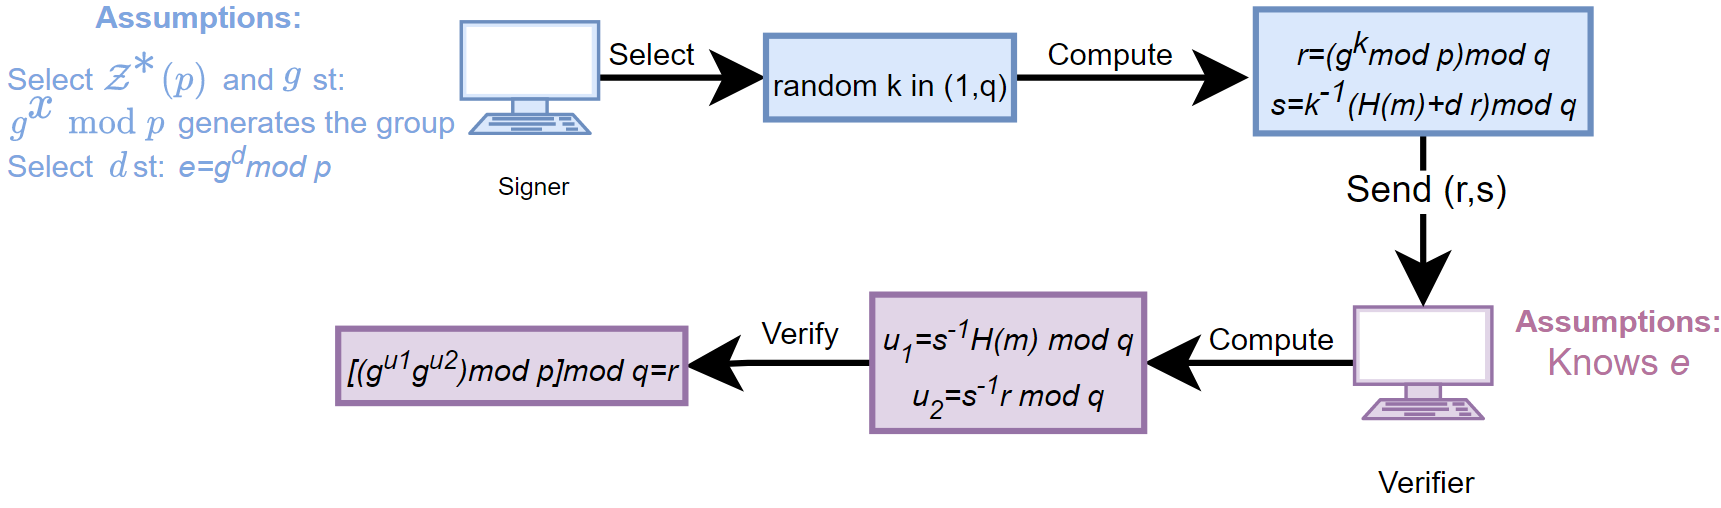
\includegraphics{image/ecc/dsa.png}
    \caption{Digital Signature Algorithm}
    \label{fig:dsa}
\end{figure}
Il processo di firma sembra robusto poiché avendo legato firma alla nonce, un attaccante non potrà replicarla. Cosa succede però se la nonce dovesse essere predicibile?\pagebreak
\begin{corollary}[Predictable Nonce in DSA]\label{cor:kpred}
Supponiamo di poter conoscere il prossimo della nonce $k$ usato per un messaggio valido (r,s)\footnotemark. Allora:
\footnotetext{\textsuperscript{\thefootnote}r ed s sono note, per questo posso risolvere l'equazione.}
\begin{align*}
    s=k^{-1}[H(m)+rd]&\longrightarrow sk=H(m)+rd\\
    d&=[sk-H(m)]r^{-1}
\end{align*}
La chiave privata è ora nota all'attaccante.
\end{corollary}
Se la nonce dovesse invece ripetersi?
\begin{corollary}[Repeated Nonce in DSA]\label{cor:krep}
Supponiamo di avere due messaggi validi $(r,s_1),(r,s_2)$ dove viene usata la stessa nonce $k$.\footnotemark\\
\footnotetext{\textsuperscript{\thefootnote}$r=(g^k\bmod p)\bmod q$. Per questo i due messaggi hanno stessa $r$}
Allora è possibile risolvere il seguente sistema:
\begin{equation*}
\begin{aligned}
    \begin{cases}
    s_1&=k{-1}[H(m_1)+rd]\\
    s_2&=k{-1}[H(m_2)+rd]
    \end{cases}
    &\longrightarrow
    \begin{cases}
    k&=s_1^{-1}[H(m_1)+rd]\\
    k&=s_2^{-1}[H(m_1)+rd]
    \end{cases}\\
    s_1^{-1}[H(m_1)+rd]&=s_2^{-1}[H(m_1)+rd]\\
    s_2H(m_1)+s_2rd&=s_1H(m_2)-s_2H(m_1)\\
d(s_2-s_1)r&=s_1H(m_2)-s_2H(m)\\
d&=[s_1H(m_2)-s_2H(m)](s_2-s_1)^{-1}r^{-1}
    \end{aligned}
\end{equation*}
\end{corollary}
\begin{remark}
Risulta evidente che la nonce $k$ \textbf{deve} essere selezionata in modo molto accurato e deve rispettare la definizione di essere \textbf{unica}, altrimenti il sistema viene completamente rotto.
\end{remark}\pagebreak
Esponiamo ora la versione di DSA sulle curve ellittiche:
\begin{definition}[Elliptic Curve Digital Signature Algorithm]\label{def:ecdsa}
\textbf{Come firmatario:}
\begin{itemize}
    \item Scelgo $E(\mathcal{Z}_p)$, con $p$ primo, $n$ (primo, \textbf{grande}) l'ordine del gruppo, $P$ il generatore del gruppo.
    \item Calcolo $Q=[d]P$, con $d$ chiave privata presa come numero \textbf{intero} $[1,n-1]$ e $Q$ la chiave pubblica.\\
    \begin{remark}
    La chiave privata è un intero, la pubblica è un punto della curva.
    \end{remark}
\end{itemize}
\textbf{Per firmare eseguo:}
\begin{itemize}
    \item Scelgo $k\in[1,n-1]$ intero casuale, \textbf{unico e NON predicibile}.
    \item Calcolo il punto $kP=(x_1,y_1)$. Le sue coordinate sono \textbf{due interi modulo p}.
    \item Per evitare che le coordinate siano \textbf{fuori dall'ordine del gruppo}\footnotemark calcolo:
    \[r=x_1\bmod n\]
    \footnotetext{\textsuperscript{\thefootnote}L'ordine del gruppo può essere più piccolo, pari o maggiore di $p$, per questo è necessario. Tuttavia, nel 99\% dei casi non si applica mai poiché $n$ non è quasi mai maggiore di $p$.}
    \item Calcolo la firma come: $s=k^{-1}(H(m)+rd)\bmod{n}$.
    \item Invio $\{m,r,s\}$
\end{itemize}
\textbf{Per verificare eseguo:} (assumendo tutti i calcoli in $\bmod{n}$)
\begin{itemize}
    \item Dal messaggio $m$ calcolo l'hash $H(m)$.
    \item Da $s$ calcolo: $w=s^{-1}\bmod n=\frac{k}{H(m)+rd}$.
    \item Calcolo (\textbf{interi}): $u_1=w\cdot H(m)$ e $u_2=r\cdot w$.
    \item Calcolo il punto della curva: $u_1P+u_2Q=(u_1+u_2d)P=(x_0,y_0)$. Ovvero:
    \begin{equation*}
        \begin{aligned}
            u_1P+u_2Q&=\frac{H(m)k}{H(m)+rd}+\frac{rk}{H(m)+rd}Q\\
            &=\frac{H(m)\cdot k}{H(m)+rd}+\frac{rd\cdot k}{H(m)+rd}P=kP
        \end{aligned}
    \end{equation*}
    \item Verifico che $v=x_0\bmod n=r$.
\end{itemize}
\begin{remark}
Lo schema è basato su Dlog e non su factoring.
\end{remark}
Vengono usati numeri primi a 256 e 384 bit per i moduli.
\end{definition}
\begin{remark}
Il motivo per il quale spesso viene riutilizzata la nonce è perché le operazioni su EC costano a livello computazionale. Sarebbe possibile quindi ottimizzare il calcolo del processo di firma calcolando $k$ una volta per tutte, ma esponendo lo schema ai problemi citati sopra.
\end{remark}
\begin{note}
Per trasferire file viene usato un algoritmo chiamato ECIES, che non vediamo in questa sede. E' usato ad esempio in 5G.
\end{note}
\begin{note}
Al giorno d'oggi, quando bisogna fare trasmissione criptata vengono usati degli HSM (Hardware Security Modules) che implementano a livello hardware algoritmi di cifratura.
\end{note}